\chapter{Background}\label{chap:background}
% \begin{algorithm}[p]
\caption{Stochastic Gradient Descent: Neural Network}
\label{alg:backpropnn}
\begin{algorithmic}
    % \ttfamily
    \State Create a mini batch of $m$ samples $\vec{x}_0 \ldots \vec{x}_{m-1}$
    \ForEach{sample $\vec{x}$}
        \State $\vec{a}^{\vec{x},0} \gets \vec{x}$  \alignedComment{Set input activation}
        \ForEach{Layer $l \in \{1\ldots L-1\}$}  \alignedComment{Forward pass }
            \State $\vec{z}^{\vec{x},l} \gets \mathbf{W}^l \vec{a}^{\vec{x},l-1}+\vec{b}^l$
            \State $\vec{a}^{\vec{x},l} \gets \varphi(\vec{z}^{\vec{x},l})$
        \EndFor
        \State $\bm{\delta}^{\vec{x},L} \gets \nabla_{\vec{a}} C_\vec{x} \odot \varphi'(\vec{z}^{\vec{x},L})$ \alignedComment{Compute error}
        \ForEach{Layer $l \in L-1, L-2 \ldots 2$}  \alignedComment{Backpropagate error}
            \State $\bm{\delta}^{\vec{x},l} \gets ((\mathbf{W}^{l+1})^T \bm{\delta}^{\vec{x},l+1})\odot \varphi'(\vec{z}^{\vec{x},l})$
        \EndFor
    \EndFor
    \ForEach{$l \in L, L-1 \ldots 2$} \Comment  \alignedComment{Gradient descent}
        \State $ \mathbf{W}^l \gets \mathbf{W}^l-\frac{\eta}{m} \sum_\vec{x} \bm{\delta}^{\vec{x},l} (\vec{a}^{\vec{x},l-1})^T$
        \State $\vec{b}^l \gets \vec{b}^l-\frac{\eta}{m}\sum_\vec{x} \bm{\delta}^{\vec{x},l}$  
    \EndFor
\end{algorithmic}
\end{algorithm}
% 
%
% \begin{figure}[t]
%     \begin{center}
%     \begin{tikzpicture}
%         \node (a) at (0,0) {a};
%         \node (b) at (2, 0) {b};
%         \draw[->] (a) -- (b);
%
%
%     \end{tikzpicture}
%     \end{center}
%     \caption[Tikz Example]{Use tikz to draw nice graphs!}
%     \label{fig:Tikz}
% \end{figure}


\section{Chromosome Conformation Capture and Hi-C}\label{sec:c3}\label{sec:hic}

\begin{figure}[t]
\begin{centering}
%    \subfloat[Diagram summarising the Hi-C experimental protocol. The red and blue rectangles represent cross-linked restriction fragments while the yellow marker shows the position of biotin incorporation.]
%    \subfloat[Generation of the Hi-C ligation junction sequence by successive digestion (with HindIII in this example), fill in and blunt-ended ligation steps. The modified restriction site sequence is not found in the original genomic sequence.]
    {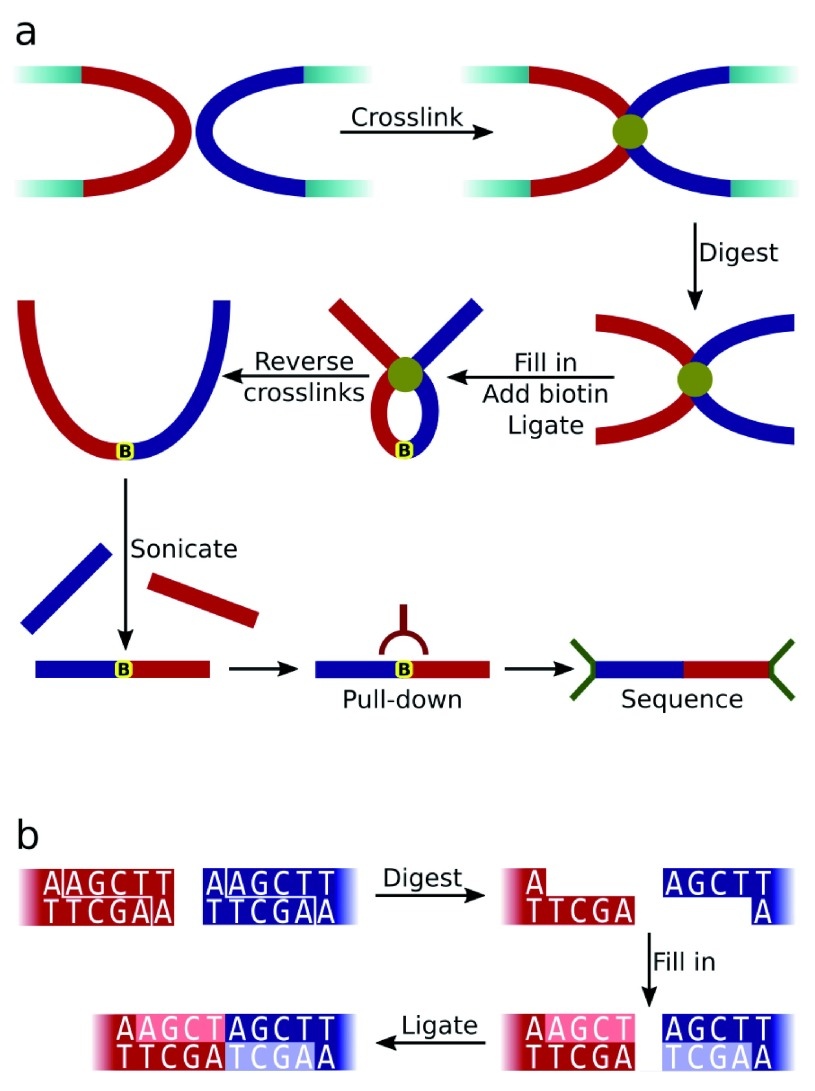
\includegraphics[scale=4]{figures/background/f1000research-4-7903-g0000.jpg}}
    \caption[Summarised Hi-C protocol]
    {\textbf{a)} Diagram summarising the Hi-C experimental protocol. The red and blue rectangles represent cross-linked restriction fragments while the yellow marker shows the position of biotin incorporation. \textbf{b)} Generation of the Hi-C ligation junction sequence by successive digestion (with HindIII in this example), fill in and blunt-ended ligation steps. The modified restriction site sequence is not found in the original genomic sequence. \\ \\ Image and description taken from \cite{wingett2015hicup}.}
    \label{fig:HiC}
    \todo{rewrite the description in my own words}

    \todo{remove the b section}
\end{centering}
\end{figure}



    % {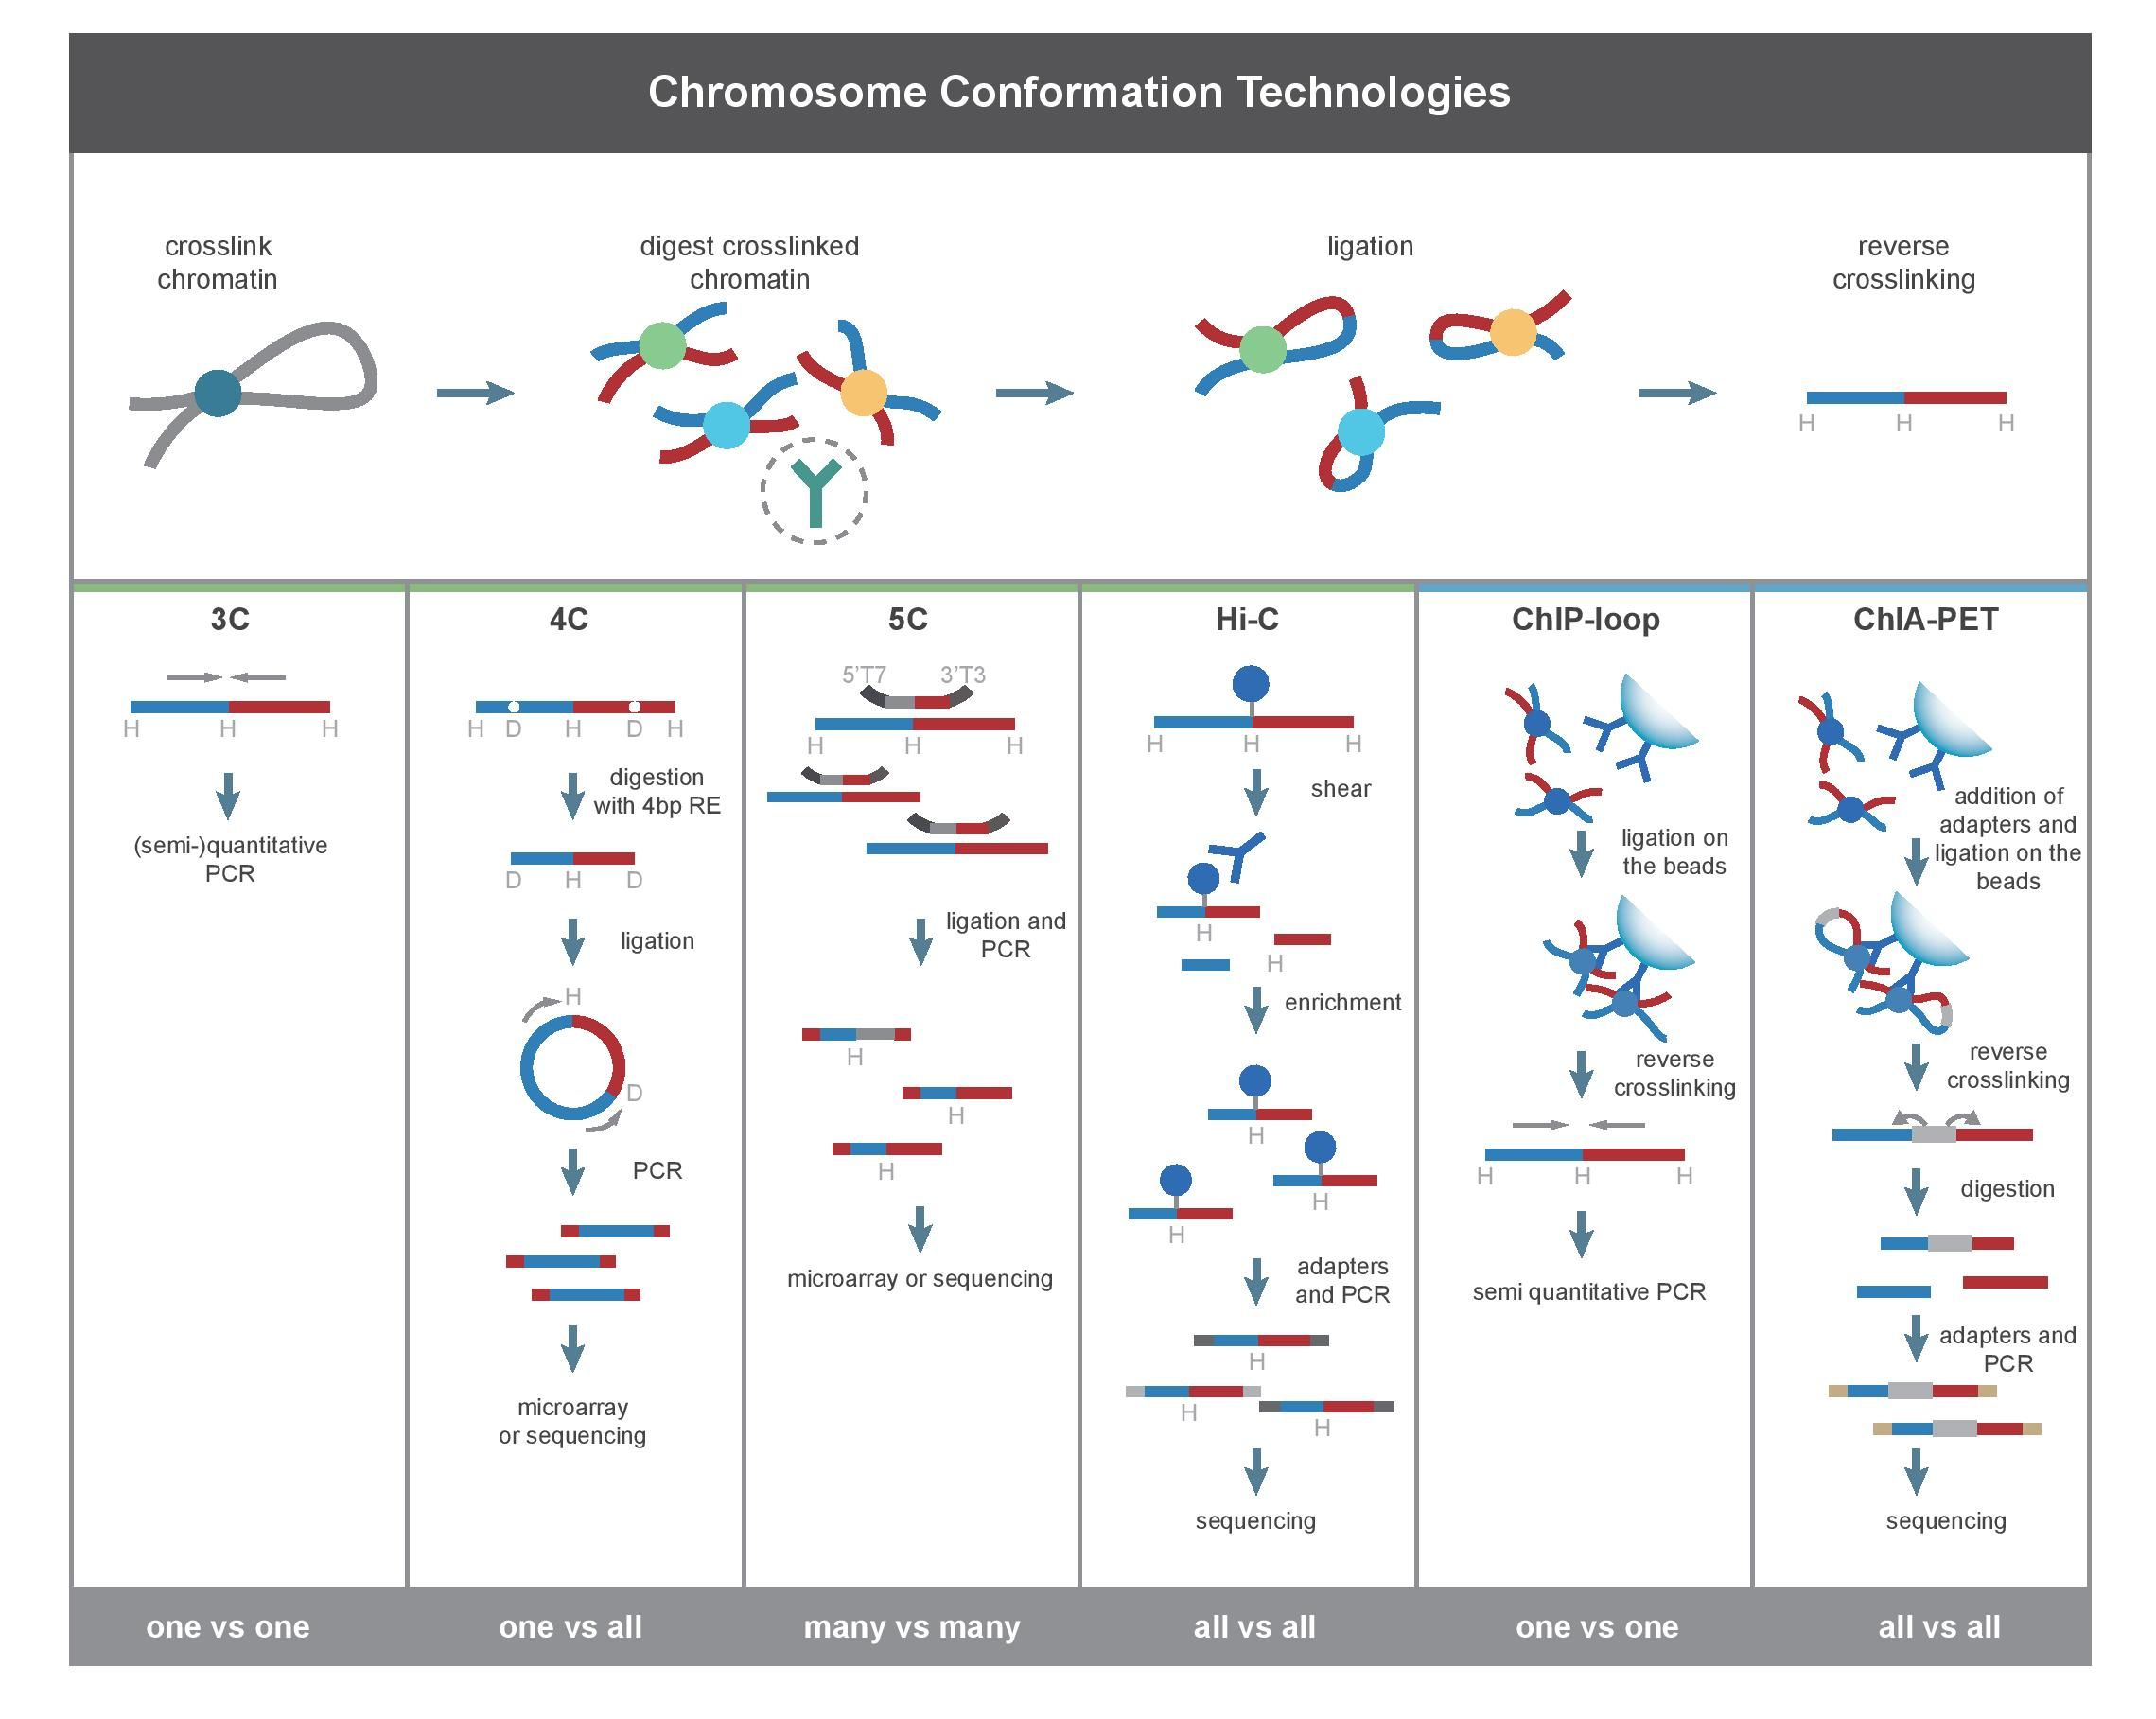
\includegraphics[scale=0.8]{figures/background/Chromosome_conformation_techniques.jpg}}
    % \caption[Comparison among 3C and its derived methods]{\textbf{Comparison among 3C and its derived methods} Source: https://en.wikipedia.org/wiki/File:Chromosome\_conformation\_techniques.jpg}


\subsection{Overview}


Chromatin usually describes different levels of how DNA organizes itself. The
well-known double-helix is only the lowest of several structural layers.

Looking at it from the outside (highest structural layer), DNA looks similar to
a big ball of wool. With the help of Hi-C (or other methods) we can visualize
the spatial proximity.

% Gene markers tend to also have effect on their spatial neighbourhood, not only on the neighbourhood going up and down the strand of DNA.



Chromosome Conformation Technologies describe several similar methods to
compare genomic loci. They all start by:

\begin{itemize}
    \item creating chromatin cross-links (\secref{sec:crosslinking}),
    \item digesting the cross-linked chromatin (\secref{sec:digestion}),
    \item ligating the ends and marking with Biotin (\secref{sec:ligation}) and
    \item reversing the cross-link (\secref{sec:revcrosslink})
\end{itemize}

to get a sequence with two parts, those parts have been spatially close
to each other and were marked with Biotin during ligation.

Other Chromosome Conformation Technologies proceed differently, Hi-C, our
focus, continues with the following steps:

\begin{itemize}
    \item shortening the cross-links by sonication (\secref{sec:sonication}),
    \item filtering leaving only those with biotin (\secref{sec:pulldown}) and
    \item sequencing (\secref{sec:sequencing}).
\end{itemize}

The full process can be seen in \figref{fig:HiC}.

\subsection{Cross-linking DNA}\label{sec:crosslinking}

The first step is to cross-link DNA strands that are close to each other
spatially (see \figref{fig:HiC} for reference). This is done by adding
formaldehyde, which bonds (links) sufficiently close strands together.

A chromatin cross-link is two entirely different parts of the genome held
together by a chemical bond with formaldehyde. This process cannot be
specifically controlled, so only `regions near each other' are connected, not
necessarily two `known to be close' regions.

\subsection{Digestion}\label{sec:digestion}

The next step is cutting the ball of wool apart in intervals. For this,
restriction-enzymes are used (specifically restriction endonuclease). Commonly
used enzymes for this are EcoR1 or HindIII, cutting the genome every 4000 base-pairs
\draft{info taken from Wikipedia, add some other source}.

This will result in a lot of cross-linked fragments, as well as not-cross-linked ones.

\subsection{Ligation}\label{sec:ligation}

After reducing the concentration of fragments, DNA ligase is added, to ligate
(weld together) dangling fragment ends. The reduction in concentration is done
since mostly fragments close together are ligated, and we intend to ligate
fragments held together by formaldehyde. Also, Biotin is added to mark the
points of ligation. This will let us filter out a lot of fragments that have
not been ligated later on.


\subsection{Reverse Cross-links}\label{sec:revcrosslink}

% Source: http://www.protocol-online.org/biology-forums/posts/10475.html
Adding a high concentration of salt for some time will reverse the
cross-linking through formaldehyde, leaving us with our two originally
spatially close fragments ligated and with a biotin-marker.

Our fragments, however, are too long to sequence them effectively (remember
that we have now ligated fragments of around 8000 base-pairs, most sequencing
methods can only deal with sequence lengths of a few hundred base-pairs).

\subsection{Sonication}\label{sec:sonication}

The next step is to put them under influence of ultrasonic waves, breaking them
apart in much shorter fragments (due to long sequences not being able to absorb
frequent shocks well), short enough to actually enable sequencing.

\subsection{Filtering and Removal of Biotin}\label{sec:pulldown}

Here we `pull-down' fragments marked with biotin, filtering all the fragments
and leaving only those having been ligated earlier (see \secref{sec:ligation}).
Subsequently we remove the marker, since it would get in the way of sequencing.

\subsection{Sequencing}\label{sec:sequencing}

Sequencing, short for DNA sequencing, describes processes of measuring a DNA
sequence. There are several techniques for doing this, most use PCR (Polymerase
Chain Reaction) before or while sequencing, which duplicates the fragments
several times, to sequence them more accurately.

% - putting the 3' and 5' ends there
% - usual PCR methods


% Open questions:
% - scaffolds?

% Chromatin is packaged into three-dimensional structures, that retain a
% relationship between genomic and physical distance. Sequences that are closer
% on the same chromosome, are also closer in physical space. Our method
% exploits this relationship between linkage and proximity to enable whole
% chromosomes scaffolding and phasing of genomes.
%
% The DNA in the sample is cross-linked in-vivo to fix DNA sequences present
% inside the same cell. Cross-linking trap sequence interactions across the
% entire genome and between different chromosomes.
%
% Cross-Linked DNA is fragmented with endonucleases. Fragmented loci are then
% biotin elated and ligated creating chimeric junctions between adjecent
% sequences. This process is called proximity ligation.
%
% The more often two sequences are joined together, the closer these two
% sequences are in genomic space.
%
% Biotinylated junctions are purified and subjected to paired-end sequencing.
% The proximity-ligation-reads are then mapped onto a draft assembly.
%
% Proximity information is used to assign context to chromosomes, and order and
% orient them along chromosome scale scaffolds.
%
% This results in fully scaffolded chromosomes of virtually any size. This
% process also detects structural variation and corrects assembly miss-joins as
% well as maps the three-dimensional conformation of chromatin within a
% population of cells.

% See \figref{fig:HiC}.


% Background:
% \todo{Cite/introduce/... the given papers, and introduce the required concepts}

% Required concepts:
% \begin{itemize}
%     \item Biology:
%     \item The iterative algorithm (again ?)
%     \item analysis that can be done further
%     \item outlook. Meaning: What can be done, when having the 3C-Data?
% \end{itemize}


% \section{Further Processing}\label{sec:furtherprocessing}

% what happens after sequencing?



\newpage

\section{deepTools}\label{sec:deeptools}

DNA sequencing is generating more data than ever before, for which deepTools,
being a framework, has useful programs to ``process the mapped reads data for
multiple quality checks, creating normalized coverage files in standard
bedGraph and bigWig file
formats''\footnote{\url{https://github.com/deeptools/deepTools}, accessed
2019-06-26} and more. Using these normalized, standardized files, many
visualizations showing the actual connections or functional
annotations, can be made.


\section{HiCExplorer}\label{sec:hicexplorer}

HiCExplorar, being part of the deepTools-framework, is a collection of tools,
that are used to process, analyze and visualize Hi-C data. Part of this
collection are tools to convert between formats, correcting the data (which
this is work is part of), normalizing it, analysing it in various ways, and
extensively plotting it. Facilitated is, among othters ``the creation of
contact matrices, correction of contacts, topologically associating domains
(TAD) detection, A/B compartments, merging, reordering or chromosomes,
conversion from different formats including cooler and detection of long-range
contacts.''\footnotemark Those contact matrices may then be visualized, also
showing other types of data, including ``genes, compartments, ChIP-seq coverage
tracks, long range contacts and the visualization of
viewpoints''\footnotemark[\value{footnote}].

\footnotetext{\url{https://github.com/deeptools/HiCExplorer}, accessed 2019-06-26}

% HiCExplorer facilitates the creation of contact matrices, correction of contacts, TAD detection, A/B compartments, merging, reordering or chromosomes, conversion from different formats including cooler and detection of long-range contacts. Moreover, it allows the visualization of multiple contact matrices along with other types of data like genes, compartments, ChIP-seq coverage tracks (and in general any type of genomic scores), long range contacts and the visualization of viewpoints.

% \begin{verbatim}
% hic2cool              hicCorrelate        hicPlotAverageRegions
% hicAdjustMatrix       hicDetectLoops      hicPlotDistVsCounts
% hicAggregateContacts  hicexplorer         hicPlotMatrix
% hicAverageRegions     hicFindTADs         hicPlotTADs
% hicBuildMatrix        hicInfo             hicPlotViewpoint
% hicCompareMatrices    hicMergeMatrixBins  hicQC
% hicConvertFormat      hicNormalize        hicSumMatrices
% hicCorrectMatrix      hicPCA              hicTransform
% \end{verbatim}

% analysing Hi-C data: building this interaction-matrix, correcting it,
% analysing it, compute stuff with it, ..., visualising the results.



\todo{was kann man tun mit den visualisierungen, und auf welche wege visualisiert man das etc?  Auf welchem Wege: Z.b. mit Software des HiCExplorer: hicPlotMatrix, hicPlotTADs, hicAggregate. Die Visualisierungen braucht man um komplexere Inhalte leichter (und vor allem schnell) verstaendlich zu machen. Niemand sieht z.B. in einer Matrizen sehr schnell hoehere Zahlenwerte, als Heatmap dagegen dargestellt sieht man sofort dass da ein anderes Muster in einem Bereich ist.  }


\todo{einführung in den HiCExplorer auf die ich verlinken könnte? Siehe eine der letzten Mails da hab ich ein Paper verlinkt.}




